An important question for cognitive science concerns the nature of mental representations. What are they, how are they structured, where do they come from, and how do cognitive processes operate on them to support behavior? One approach to cognition, variously referred to as the parallel distributed processing (PDP), connectionist, or neural network approach, has offered fairly specific answers to these questions \cite{McClellandRumelhart86}. It begins with the central tenet of cognitive neuroscience that all cognitive processes ultimately arise from the propagation of activity amongst large populations of neurons communicating their states via excitatory and inhibitory synaptic connections; but it further proposes that the important characteristics of such systems can be captured in simplified abstract form by computer models that simulate the flow of information through networks of neuron-like processing units connected by weighted synapse-like connections. All cognitive abilities are proposed to arise from representational and processing mechanisms that can be so described and understood. Accordingly, the framework offers a constrained view of what mental representations are: patterns of neural activity evoked by a stimulus or a process over a set of units operating in parallel. Often such representations are proposed to be highly distributed, so that (1) any given unit contributes to the representation of many different items, (2) any given item representation is encoded over many different units and (3) the representation inheres in the full pattern of activation over all units, and not in the activation of individual units.

Distributed representations of this kind have several properties that make them useful for understanding various aspects of cognition. For instance, they provide a natural basis for similarity-based generalization \cite{hinton_distributed_1984,RumelhartTodd93}. Two different items that generate overlapping patterns of activation over the same units will tend to produce similar responses downstream in the network. Thus distributed representations explain how prior learning supports the processing of novel inputs, an ability central to accounts of categorization, inductive inference, language processing, and many other cognitive phenomena. Similarity-based generalization also naturally produces patterns of behavior observed in many different tasks, such as typicality effects, frequency effects, and effects of quasi-regularity \cite{plaut_understanding_1996,rogers_semantic_2004}. Distributed representations explain why, with neuropathology, cognitive abilities are not disrupted in an all-or-none fashion, but instead degrade gracefully: when some units in the representation are destroyed or disrupted, the remaining units continue to communicate with downstream units, transmitting information that may still be at least approximately correct \cite{Allport85,cooper_shallice_2011}. They provide a means of understanding the acquisition of new representations: rather than adding new information to a database, or new representational elements into a processing system, new representations can be acquired by adjusting connections within the network so that a given stimulus or process generates a new pattern of activity over the existing units \cite{RumelhartTodd93}. Finally, distributed representations can be highly efficient. With a local code, in which each unit represents one and only one item of information, then with n units it is possible to represent just n items. With a binary distributed coded, the same n units can represent $2^n$ distinct items; and if the units encode continuous activation values there is, in principle, no limit to the number of items a given set of units can encode \cite{hinton_distributed_1984}.

These virtues are well known and form the basis for influential accounts of healthy, disordered, and developing cognition in theories of reading \cite{seidenberg_distributed_1989,harm_computing_2004}, inflectional morphology \cite{RumelhartMcClelland86pt,JoanisseSeidenberg99, plunkett_connectionist_1999}, semantic processing \cite{FarahMcClelland91,rogers_semantic_2004,rogers_structure_2004}, routine sequential action \cite{BotvinickPlaut2004} and many other domains \cite<see>[for a recent review]{rogers2014parallel}. Perhaps surprisingly, however, remarkably little work in cognitive neuroscience has attempted to directly test PDP's assumptions about the neural basis of mental representations. The reasons for this gap are probably methodological, at least in part. The most ubiquitous methods in human cognitive neuroscience---fMRI and other functional brain imaging technologies---typically yield vast amounts of noisy data.  To discern interesting patterns in these datasets, or to test particular hypotheses, the statistical models employed must adopt specific assumptions about the nature of the underlying signal. For many years, standard statistical approaches were built upon representational assumptions that were at odds with those adopted under the PDP approach \cite{kriegeskorte_representational_2008}. As a result it has been difficult to relate the results of such analyses to the predictions of PDP models. This has begun to change with the advent of new multivariate methods for analyzing brain imaging data but many challenges still remain. Several different approaches have appeared in the literature in recent years \cite{pereira_machine_2009,kriegeskorte_information-based_2006,kriegeskorte_representational_2013,mitchell_predicting_2008}, %\orange{references to Poldrack here and others here?} 
each carrying with it particular assumptions about the nature of the underlying neural code, and so bringing biases in the kind of signal it is capable of detecting. Moreover, the nature of the assumptions and their implications for measuring neural representations may not always be completely transparent, although important work is being done to address this \cite<e.g.,>{davis_measuring_2013}. Thus, although the PDP framework and related approaches put forward quite specific hypotheses about the nature of representations in the mind and brain, it has not been clear how neuroscientific methods, and in particular functional brain imaging, might best be leveraged to test these hypotheses.

The goal of the current paper is to consider how the analysis of brain imaging data might best be approached if the PDP assumptions about mental representation are valid. We first consider in more detail what the PDP assumptions are and why they pose challenges for standard and even many state of the art brain imaging methods. To illustrate these points, we compare and contrast the results yielded by five different statistical methods in the analysis of the activation patterns generated by different inputs to a simple PDP model.  Since the behavior, architecture, and representational structure embedded in the simple model are fully known, it is possible to measure the extent to which the various methods succeed in identifying the model components that encode interesting representational structure. This analysis thus illustrates the strengths and weaknesses of different approaches if PDP assumptions about representation are valid. The results suggest a new strategy for the analysis of functional imaging data that may help to better connect PDP models to cognitive neuroscience. We then assess the utility of this approach by comparing its results to those of other state of the art methods in the analysis of one well-known publicly released fMRI dataset.

% We take the activation of a single unit as a model analog of the mean activity in a population of neighboring neurons, similar to that estimated from changes in the BOLD response at a single voxel.

\section{A brief overview of PDP models and their representational assumptions}
PDP models are composed of simple processing units that communicate via weighted synapse-like connections \cite{McClellandRumelhart86,rogers2014parallel}.
Each unit adopts an activation state, typically varying between 0 and 1, that can be viewed as analogous in some respects to the mean firing rate of a population of spiking neurons proportional to their maximal rate \cite{ZipserAndersen88}. Units transmit information about their current activation through weighted connections, which can be viewed as capturing the net effect of activity in one population of neurons on another. Weights are typically real-valued, with negative numbers indicating a net inhibitory effect and positive numbers indicating a net excitatory effect. Each unit computes a simple process: it adjusts its current activation state according to the input it receives from other units in the networks. If a given receiving unit receives inputs from a set of $n$ sending units, then the input is usually computed as the inner product of the activation across all sending units and the values of the weights projecting from the sending units to the receiving units. The unit then converts the net input into a new activation state according to a specified transfer function (often a sigmoid function of the net input). All units are conceived as computing inputs and updating activation states in parallel in continuous real time (hence ``parallel'' distributed processing), though on serial computers this parallel process is simulated by updating units in discrete steps in randomly permuted order.

Within a network, units are generally organized into layers, which govern the overall connectivity of the network: units within a layer tend to receive connections from, and direct connections toward, a similar set of units elsewhere in the network. Typically a subset of the units are specified to receive inputs directly from sensory systems (or other input systems outside the model), and to direct outputs toward motor systems (or other output systems outside the model). These unit subsets encode the input provided to the model and the outputs that simulate the model response. They are often referred to as {\em visible} units, because the theorist directly stipulates how different stimulus events and behaviors are represented with patterns of activation over the input and output units. Most models also include sets of units whose inputs and outputs are directed only to other units contained within the model---they do not receive external inputs from or direct outputs toward the model environment. For these {\em hidden} units, the theorist does not stipulate how different stimulus events or behaviors are to be coded with patterns of activation. Instead, the patterns of activation that arise across these units are determined solely by the values of the interconnecting weights. 

The weights themselves are viewed as being shaped by learning and experience. Many different learning algorithms have been explored in this framework \cite<see>{hinton2014where}, but all share the general idea that the weights gradually change over time in order to optimize some objective function---for instance, minimizing the discrepancy between the outputs the model generates and the correct ``target'' outputs---as the network processes information from different stimulus events. Because the weights adapt to experience, and because the patterns of activation over hidden units depend upon the weight values, PDP models are therefore capable of acquiring learned internal representations: the patterns of activation generated over hidden units by a given stimulus after the network has undergone learning in a model environment.  One interesting aspect of PDP models, responsible for their utility in many different cognitive domains, concerns the nature of the internal representations they acquire after learning in a structured environment. Often the models can acquire internal representations that may seem counter-intuitive from other points of view, but that can be shown, through computer simulations, to support behaviors documented in the domain of interest. Figure \ref{fig.sem_net} and its caption provide one example of a PDP model used to understand aspects of semantic memory.

\begin{center}
\textbf{---Figure \ref{fig.sem_net} about here---}
\end{center}


\begin{figure}
\centering
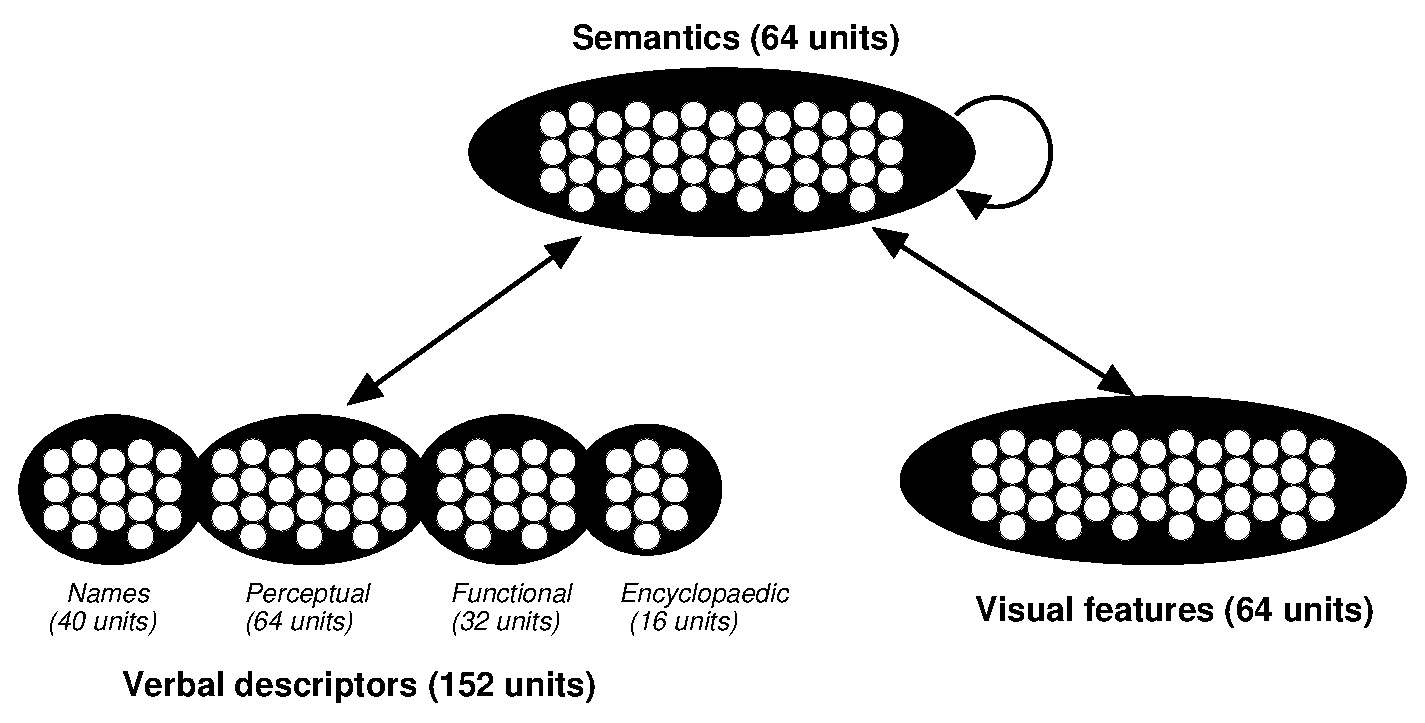
\includegraphics[width=0.70\textwidth]{figures/figure1.eps}
\caption{ A PDP model used to understand semantic memory (from \protect\citeNP{rogers_structure_2004}). Units in the {\em Visual} layer code visual features and units in the {\em Verbal} layer encode familiar words. The {\em Visual} and {\em Verbal} units can receive direct inputs from the environment, corresponding to direct perception of a visually-presented item or of a spoken statement. Units in both layers send connections to, and receive connections from, an intermediating hidden layer. To simulate a task such as object naming, visual features of the object are directly activated in the {\em Visual} layer and the activation propagates to other units via the weighted connections. If the weights are set to appropriate values, the model will ultimately activate the {\em Verbal} unit corresponding to the item name. Likewise name comprehension is simulated by directly activating the unit corresponding to the name and propagating activation throughout the network. With appropriate weights the visual features of the named item will activate, along with verbal units describing the item's properties.  Appropriate weights are discovered through a predictive error-driven  learning algorithm. Following learning, each input provokes a pattern of activation over hidden units that depends on the acquired weight configuration---a learned internal representation of the input. Though the particular pattern acquired for a given item varies across training runs, the representations always encode the same similarity structure among items in the environment, representing items that are conceptually related with similar patterns of activation.}
\label{fig.sem_net}
\end{figure}

With this overview of how PDP models work, we are ready to consider the challenges that the framework raises for the discovery of mental representations in functional brain imaging data. Many difficult issues arise, of course, in any effort to relate artificial neural networks to real neural networks. Because network models are functional abstractions of the neural processes they aim to uncover, they necessarily gloss the complexity, and many aspects of structure and behavior, known to be important in real nervous systems. Whereas individual neurons exhibit all-or-nothing spiking behavior, model units assume continuous activation states. Low-level dynamics such as lateral inhibition, temporal coherence, and local extra-cellular conditions are glossed over in most connectionist models, while morphological differences among neuron types, cytoarchitecture, and other facts about brains are completely abstracted away. PDP units can instead be viewed as capturing, in a modest number of processing elements, the same informational states existing across vast numbers of heterogeneous spiking neurons in real nervous systems \cite{Smolensky86,rogers2014parallel}. The central assumption is that the representational content and cognitive functions expressed in the coordinated spiking behaviors of hundreds or thousands of neurons can be usefully approximated as a much smaller vector of continuous-valued activations. As we have noted elsewhere \cite{Cox2014}, this is essentially the same assumption adopted in fMRI and other brain imaging methods which summarize the dynamical activity over hundreds of thousands of neurons at a millisecond timescale with a much smaller vector of real-valued numbers, each expressing the overall metabolic demands exerted by populations of neurons within a $3mm^2$ voxel. The effort to relate neural activity to cognitive events entails the assumption that important informational states over vast sets of neurons can be so abstracted. 

We therefore adopt here a fairly simplified stance on the relationship between network models and the brain networks we seek to discover in imaging data. Specifically, we assume that the activation of a single unit in a network model is roughly analogous to mean neural activity in a population of hundreds of neighboring neurons within a small volume of cortex as estimated at a single voxel from BOLD activity in fMRI. Thus we will treat the pattern of activation generated by a given stimulus over units in a model network as analogous to the set of beta coefficients estimated over voxels from the BOLD response evoked by a given stimulus in a sparse event-related design. 

Even with this relatively transparent view of the relation between model elements and measured physiological responses, PDP raises four difficult challenges for the discovery of representational structure in the brain.

%\begin{APAenumerate}
{\em 1. The behavior of a given cortical subregion (i.e., voxel or voxel cluster) can vary substantially across individuals even if different individuals encode the same representational structure across the same general regions.} For any given network, there are typically many different weight configurations that can generate appropriate outputs given the various inputs. The particular configuration that a network discovers with learning can depend on many things, including the initial random weight configuration, the ordering and distribution of the learning experiences sampled from the environment, and the effects of noise in the unit activations and/or weight changes. Thus a particular hidden unit in a given model can, across different training runs in the exact same environment, exhibit quite different patterns of activation in response to a given input. Yet the internal representations learned by a network are not arbitrary; the learning models are of interest because they reliably extract important similarity structure across the set of input and output patterns to which they are exposed. What varies is the particular way that individual units contribute to encoding the interesting structure across network runs. \citeA{Cox2014} provide a simple example of this kind of variability in a simple model.

We can conceive of a single model training run as simulating the effects of learning and experience in a single individual person. The different weight configurations and internal codes that arise across model training runs thus indicate the kind of variability in representation that may exist across individuals under the PDP view, even if the individuals show the same pattern of overt behavior in the domain and the same gross neural architecture. Specifically, the response generated by a given stimulus or process in a given patch of cortex may vary arbitrarily across individuals,  even if the same representational structure is being encoded across the same cortical subregions. This possibility poses a challenge to imaging methods that focus on finding voxel clusters that reside in similar locations and respond in similar ways across individuals. If representations vary across individuals in the way that PDP models suggest, such methods will fail to discover them.

This consequence of distributed representations may pose greater problems for finding signal in some cortical regions than others. In peripheral regions (i.e., early sensory and motor cortices), it is clear that information is encoded in largely the same way, and with a largely similar neuroanatomical organization, across individuals. In association cortices, it may be that neural codes are less constrained are more strongly shaped by learning and experience, so that the way information is organized across cortex is more highly variable. PDP models provide a rough analog to this state of affairs, insofar as input and output units for a given model are stipulated to represent information in the same way in every model training run---that is, in every model ``individual.'' The issues of variability in representation mainly apply to learned internal representations coded across hidden units.

{\em 2. Activation of individual units may not be interpretable independent of other units.} A corollary of the preceding points is that the behavior of a given cortical unit may not be interpretable, or may have quite different interpretations across individuals, when analyzed independently from other units. This property of distributed representation is important because it suggests that univariate approaches to data analysis---methods that assess the behavior of individual voxels or voxel clusters independently---can fail to uncover important components of neural representations. Wherever the interesting structure is embedded in activations across multiple cortical units, but is not reflected in individual units, such methods will yield null results \cite<see>[for a concrete example]{Cox2014}. 

{\em 3. The functional model architecture may not map transparently onto anatomical structure in the brain.} A third issue concerns the relationship between the functional architecture of a computational model used to simulate performance on a task of interest and the actual anatomical structure of the corresponding neural network in the brain.  As noted earlier, units in PDP models are organized into layers, with units in a given layer receiving connections from and directing connections toward the same subsets of units elsewhere in a network. The layer is a useful construct for understanding how a network functions, insofar as the units within a layer, by virtue of having similar connectivity to the broader network, ``work together'' to represent and process the same information. Distributed internal representations in PDP networks are typically viewed, therefore, as being encoded across units within a particular layer.  

It may seem natural to view layers as model analogs of cortical regions, so that the gross architecture of a computational model maps transparently onto the anatomical structure of networks in the brain that carry out the modeled cognitive function. Though this analogy is reasonable, it is not the only possible way that the functional architecture of a computational model might relate to the neuroanatomical structure of a corresponding cortical network. In fact, the layers of a computational model do not, in principle, have any implications for how the corresponding cortical units might be anatomically situated in the brain. Units that function together as a ``layer'' could be situated in multiple different cortical regions, or widely dispersed anatomically, or interdigitated with other units subserving different functions. The defining property of layers in a computational model is their pattern of connectivity in the gross architecture, and the same network connectivity can exist among many different spatial arrangements of units. In other words, the relationship between the functional architecture of a computational model---the grouping of units into layers as typically depicted in model figures, for instance---may not transparently reflect the topological arrangement of the corresponding cortical units in the brain. 

This lack of transparency poses a problem for approaches to brain imaging that assume representations to be encoded over a volume of anatomically contiguous cortical units, including approaches that average signal over regions of interest, that spatially blur signal, or that restrict statistical analysis only to voxels within pre-specified areas. If cortical units that function together as a representational substrate do not happen to reside in a single contiguous cortical region, such methods may fail to discover important signal.

This is not to suggest that the PDP view predicts that anatomical structure is unimportant, or that shared structure across individuals is unexpected or meaningless. To the contrary, the connectivity of a given network strongly constrains its behavior. Thus the network architecture always constitutes an important aspect of the explanatory hypothesis a model is intended to exemplify. It is typically assumed that this architecture is largely shared across individuals, and that, however it is anatomically situated in the brain, there will be at least coarse similarities across individuals. 

{\em 4. The network of interest in any given study co-exists in the brain with many other networks, all subserving other functions that may not be of interest.} Any given computational model is designed to aid understanding of a particular aspect of cognition, and typically includes only those elements that the theory stipulates to be important for the behavior of interest. Even if the model is a relatively faithful and accurate abstraction of a real cortical network in the brain, the physiological measurements generated by that network will be intermingled with measurements from a great many other cortical systems involved in other aspects of cognition unrelated to the task of interest. Odds are that the great majority of measurements taken will reflect metabolic activity unrelated to the representational structure we are searching for. Thus the effort to find distributed representations in brain imaging data raises concerns about needles and haystacks. 

%\end{APAenumerate}

\subsection{Summary}
The representational assumptions of the PDP framework lead to rather bleak outlook. The behaviors of individual cortical units (i.e., voxels) may not independently covary with or otherwise reflect the objects of representation we are interested in finding in a systematic way across individuals. Mental representations may instead inhere in the patterns of activation evoked across whole sets of units that together function as a representational ensemble by virtue of their connectivity within the overall cortical network (like the layers of a neural network model). This is the core sense in which representations are distributed in the PDP view. The way that a particular unit contributes to different representations can be highly variable across individuals, even if the ensemble encodes the same representational structure across individuals. This means that the search for voxels exhibiting similar responses in similar anatomical locations across people will fail to reveal important representational structure. Moreover, the units that operate together as a representational ensemble may not be anatomical neighbors, may vary in their location to some extent across individuals, and are certain to be buried within the mountain of measurements provided by functional imaging technologies across the whole brain. These possibilities raise a daunting challenge: representational structure can only be discerned by considering the whole pattern of activation over a representational ensemble; yet the units within such an ensemble may be anatomically dispersed and intermingled with a vast amount of irrelevant information. One cannot understand the representation without knowing which units together constitute an ensemble, but how is one to find the ensemble in the first place?

In what follows, we assess how well different approaches to fMRI data analysis meet this challenge by applying them to the discovery of representational structure in data generated by a simple neural network model as it processes different input patterns. We will see that all methods bring with them important biases in the kinds of representational structure they are capable of detecting, and that some methods are better-suited to finding the distributed structure that the PDP framework assumes. We will also see that patterns of results across methods can provide important information about the nature of the representations encoded in different parts of a network.

